\documentclass[twoside]{article} 
\usepackage{amsmath}
\usepackage{amsfonts}
\usepackage[pdftex]{graphicx}
\usepackage[procnames]{listings}
\usepackage{color}
\usepackage{lipsum} % Package to generate dummy text throughout this template
\usepackage{braket}
\usepackage{epsfig}
\usepackage{epstopdf}


\usepackage[sc]{mathpazo} % Use the Palatino font
\usepackage[T1]{fontenc} % Use 8-bit encoding that has 256 glyphs
\linespread{1.05} % Line spacing - Palatino needs more space between lines
\usepackage{microtype} % Slightly tweak font spacing for aesthetics

\usepackage[hmarginratio=1:1,top=32mm,columnsep=20pt]{geometry} % Document margins
\usepackage{multicol} % Used for the two-column layout of the document
\usepackage[hang, small,labelfont=bf,up,textfont=it,up]{caption} % Custom captions under/above floats in tables or figures
\usepackage{float} % Required for tables and figures in the multi-column environment - they need to be placed in specific locations with the [H] (e.g. \begin{table}[H])
\usepackage{hyperref} % For hyperlinks in the PDF

\usepackage{lettrine} % The lettrine is the first enlarged letter at the beginning of the text
\usepackage{paralist} % Used for the compactitem environment which makes bullet points with less space between them

\newcommand{\unit}[1]{\ensuremath{\; \mathrm{#1}}}

\usepackage{abstract} % Allows abstract customization
\renewcommand{\abstractnamefont}{\normalfont\bfseries} % Set the "Abstract" text to bold
\renewcommand{\abstracttextfont}{\normalfont\small\itshape} % Set the abstract itself to small italic text

\usepackage{titlesec} % Allows customization of titles
\renewcommand\thesection{\arabic{section}} % Roman numerals for the sections
\renewcommand\thesubsection{\thesection.\arabic{subsection}} % Roman numerals for subsections
\titleformat{\section}[block]{\large\scshape\centering}{\thesection.}{1em}{} % Change the look of the section titles
\titleformat{\subsection}[block]{\large}{\thesubsection.}{1em}{} % Change the look of the section titles

\usepackage{fancyhdr} % Headers and footers
\pagestyle{fancy} % All pages have headers and footers
\fancyhf{}
\fancyhead[C]{Molecular Dynamics Simulation of a Lenard-Jones Interacting Molecule for Obtaining Macroscopic Static Physical Properties $\bullet$ February 2016} % Custom header text
\fancyfoot[RO,LE]{\thepage} % Custom footer text
\fancyfoot[CO,CE]{Jaap Wesdorp \& Bas Dirkse}
\fancypagestyle{firststyle}
{	
	\fancyhf{}
	\renewcommand{\headrulewidth}{0pt}
	\fancyfoot[RO,LE]{\thepage}
	\fancyfoot[CO,CE]{Jaap Wesdorp \& Bas Dirkse}
}

\usepackage{subcaption}
\captionsetup{compatibility=false}

%----------------------------------------------------------------------------------------
%	TITLE SECTION
%----------------------------------------------------------------------------------------

\title{\vspace{-15mm}\fontsize{18pt}{10pt}\selectfont\textbf{Molecular Dynamics Simulation of a Lenard-Jones Interacting Molecule for Obtaining Macroscopic Static Physical Properties}} % Article title

\author{
	\large
	\textsc{Jaap Wesdorp}$^\dagger$, $\hspace{10pt}$ \textsc{Bas Dirkse}$^\dagger$ \\ % Your name
	\normalsize $^\dagger$Delft University of Technology \\ % Your institution
	\normalsize \href{mailto:j.j.wesdorp@student.tudelft.nl}{j.j.wesdorp@student.tudelft.nl} \\
	\normalsize \href{mailto:b.dirkse@student.tudelft.nl}{b.dirkse@student.tudelft.nl} 
}
\date{\today\vspace{-8mm}}

%----------------------------------------------------------------------------------------

\begin{document}

\definecolor{keywords}{RGB}{255,0,90}
\definecolor{comments}{RGB}{0,0,113}
\definecolor{red}{RGB}{160,0,0}
\definecolor{green}{RGB}{0,150,0}

\lstset{language=Python, 
	basicstyle=\ttfamily\small, 
	keywordstyle=\color{keywords},
	commentstyle=\color{comments},
	stringstyle=\color{red},
	showstringspaces=false,
	identifierstyle=\color{green},
	procnamekeys={def,class}}

\maketitle % Insert title
\thispagestyle{firststyle} % Only footer on first page

%----------------------------------------------------------------------------------------
%	ABSTRACT
%----------------------------------------------------------------------------------------

\begin{abstract}
\noindent  
The equations of motion for 864 particles have been integrated using the Lenard-Jones pairwise interaction potential to model the particle interaction. We have simulated for several densities and at several temperatures, obtaining macroscopic quantities of argon for the relevant state. The heat capacity and constant volume was confirmed to agree with theoretical results and isotherms were computed in a pressure-density plot. Finally we have computed the pair correlation function, showing that the Lenard-Jones interaction works well to model argon in the gas, liquid and solid phase.

	
\end{abstract}

%----------------------------------------------------------------------------------------
%	ARTICLE CONTENTS
%----------------------------------------------------------------------------------------

\section{Introduction}

\lettrine[nindent=1em,lines=2]{I}
n this paper we intend to derive experimental macroscopic properties of a material from a microscopic description of the molecular interactions. In statistical physics many macroscopic quantities of many-particle systems can be found as an ensemble average over the possible microscopic states. Any practical macroscopic system consists of so many possible microscopic states that it is infeasible to average over all of the possible states computationally. But given a large subset of the possible states, we may assume that physical quantities averaged over the subset are close to the ensemble average. In molecular dynamics (MD) we initialize a specific state determined by some system parameters and let it evolve in time, traversing along its physical trajectory in the phase space as determined by the equations of motion. We therefore generate a large subset of possible states which are correlated in time. Using appropriate averaging over time we can obtain estimates of the ensemble average and therefore the relevant physical quantities.

We restrict ourselves to studying static physical properties of the system at equilibrium, although MD could also be used to study dynamical properties of a system. We carry out simulations for Argon, which is studied extensively in the literature and is modeled easily using the Lenard-Jones interaction potential. First we compute the heat capacity and compare it to theoretical results in the case of a hot and dilute gas or a cold and dense solid to verify the result. Next we compute the pressure as a function of the density at different temperatures and compare this with experimental results. Finally we compute the pair correlation function and comment on its qualitative behavior.

%------------------------------------------------

\section{Methods}
\subsection{Molecular Dynamics and the interaction potential for Argon}
For the simulation a box of fixed dimensions $L\times L\times L$ is considered containing $N$ particles obeying periodic boundary conditions. During the simulation we keep track of the particle positions $\mathbf{r}_i$ and particle velocities $\mathbf{v}_i$. At each time step we calculate the total force on each particle $i$ due to the interaction potential $U(\mathbf{r}_i,\mathbf{r}_j)$ with all other particles $j$.  
We assume only pairwise interaction between the particles and that this interaction only depends on the distance between particles $r_{ij} = | \mathbf{r}_i - \mathbf{r}_j |$. An interaction potential that works particularly well for argon is the Lennard-Jones potential which is given by
\begin{equation}\label{eq_lj}
U_{LJ}(r) = 4\epsilon \left[\left(\frac{\sigma}{r}\right)^{12} - \left(\frac{\sigma}{r}\right)^6  \right].
\end{equation}
The total force  $\mathbf{F}_i$  on a single particle $i$ is then given by 
\begin{equation}\label{eq_force_sum}
\mathbf{F}_i = -\sum_{j\not=i}^N \left.\frac{\partial u_{LJ}}{\partial r}\right|_{r= |\mathbf{r}_{ij}|}  \frac{\mathbf{r}_{ij}}{|\mathbf{r}_{ij}|}
\end{equation}
We neglect any external forces, resulting in the following equations of motion of the $N$ particles
\begin{equation}\label{eq_motion}
\frac{\partial ^2\mathbf{r}_i}{\partial t^2} = \frac{\mathbf{F}_i}{m_i} \hspace{20pt} i\in [1, N]
\end{equation}

\subsubsection*{Discretisation: Verlet Algorithm}

The simulation is performed using time steps of size $\Delta t$, the equations of motion are then discretised using the Verlet algorithm \cite{ref_verlet}. For the position vectors we get
\begin{equation}\label{eq_verlet_pos}
\mathbf{r}_i(t+\Delta t) = \mathbf{r}_i(t) + \mathbf{v}_i(t)\Delta t + \frac{\mathbf{F}_i}{m}(\Delta t) ^2,  \hspace{20pt} i\in [1, N],
\end{equation}
and for the velocity at $T+\Delta t$ we get
\begin{equation}\label{eq_verlet_vel}
\mathbf{v}_i(t+\Delta t) = \mathbf{v}_i(t) + \Delta t \frac{\mathbf{F}_i(t + \Delta t) + \mathbf{F}_i(t)}{2m},  \hspace{20pt} i\in [1, N].
\end{equation}

\subsubsection*{Periodic Boundary Conditions}
After each coordinate update, we need to check if the particles still reside within the boundaries of the box. If this is not the case we use periodic boundary conditions to translate the particles by the box length $L$ back in the box. These periodic boundary conditions can be applied separately in each dimension, so for a single dimension x we get the following update rule for the position of a single particle
\begin{equation}\label{eq_pbc}
r_x \rightarrow r_x \mod{L}
\end{equation}
And the same holds for the $y$ and $z$ coordinates of the particle. These boundary conditions are also applied in the force calculation by the sum of \eqref{eq_force_sum}, where the closest image of the particle $j$ with respect to particle $i$ is chosen to be used, since that gives the largest contribution to the force. Indeed, if $L > 5\sigma$ then all other images of particle $j$ are further away from particle $i$ than the typical cutoff distance of $2.5\sigma$ for the Lenard-Jones potential and therefore their contributions to $\mathbf{F}_i$ can be neglected.


\subsubsection*{Initial conditions}
Solid argon at low temperatures and high density is experimentally seen to form an FCC lattice. The FCC is an orthorhombic lattice containing four particles per unit cell. If we assume the first particle to be located at position $(0,0,0)$ the others are located at $(0,\frac{1}{2},\frac{1}{2})$, $(\frac{1}{2},0,\frac{1}{2})$, $(\frac{1}{2},\frac{1}{2},0)$ if the unit cell has length 1. We use these positions as initial positions for the particles.

For the initial velocity we use the fact that the probability of a particle having a certain kinetic energy $K$ is given by the boltzmann weight 
\begin{equation}\label{eq_boltzmann}
P(K_i) \sim e^{\frac{-|\mathbf{v}_i|^2}{2T}}
\end{equation}
From this we can see that each component of $\mathbf{v}_i$ is normally distributed with mean zero and standard deviation equal to $\sqrt{T}$, where we used the natural units described in the next section. Due to the finite amount of particles, sampling from the normal distribution with mean zero will in general not result in a zero mean velocity. To compensate for this we subtract the residual mean velocity after sampling ensuring that there is no net momentum.  


\subsubsection*{Natural Units of Computation}
Since the Lennard-Jones potential(\eqref{eq_lj}) is based on two parameters $\sigma [m]$ and $\epsilon [J]$, we define our distance in units of $\sigma$ and energy in units of $\epsilon$. For the total SI system to be written in these natural units we need a third unit, so let's take the mass $m$ equal to one (the unit of mass is thus the argon atomic mass). The temperature will then be expressed as $T  = \epsilon/k_B$. These choices will also defines the unit of time as $\tau = \sqrt{m\sigma^2/\epsilon}$. This generalizes our model to any molecule obeying the LJ potential and forms a FCC lattice structure. If the units have to be transformed back to SI units one can simply fill in the literature values of $\epsilon$, $\sigma$ and $m$ for the specific material. For argon these values are $\epsilon_{Ar} = 120 \unit{k_B}$, $\sigma_{Ar} = 0.34 \unit{nm}$ and $m_{Ar} = 39.95 \unit{\frac{g}{mol}}$ where $k_B$ is Boltzmann's constant. So a temperature $T = 1$ in our simulation for argon would then correspond to $T = 120 \unit{K}$ in SI units. For argon, we also find $\tau \approx 2.15 \cdot 10^{-15} \unit{s}$.

\subsubsection*{The (N, V, E) and (N, V, T) ensemble}
Since we allow for a random initial kinetic energy $K$ and then conserve the total energy, we effectively simulate the micro-canonical ensemble (N, V, E). It is also possible to simulate the canonical ensemble (N, V, T). This amounts to our system being surrounded by a large heat bath of constant temperature. In this ensemble we therefore need the kinetic energy to remain constant. This can be achieved by rescaling the velocity at each time step as to remain at a constant kinetic energy corresponding to the temperature $T$
\begin{equation}\label{eq_vel_rescale}
\mathbf{v}_i \rightarrow \sqrt{\frac{3 T}{\frac{1}{N} \sum_{j=1}^N |\mathbf{v_j}|^2}} \mathbf{v}_i
\end{equation}


\subsection{Computation of physical quantities}
\subsubsection*{Computation of the heat capacity}
Computing the heat capacity at constant volume can be done in the canonical ensemble using the partition function, which can ultimately be related to the rms-fluctuations of the total energy. However in this paper, we wish to compute the heat capacity at constant volume in the microcanonical ensemble. In the microcanonical ensemble, the heat capacity at constant volume can be computed from the rms-fluctuations in the kinetic energy using a formula derived by Lebowitz\cite{ref_Lebowitz} 
\begin{equation}
\frac{\braket{K^2} - \braket{K}^2}{\braket{K}^2} = \frac{2}{3N} \left( 1 - \frac{3N}{2C_V} \right),
\label{eq_Lebowitz}
\end{equation}
where $K$ denotes the kinetic energy, and $N$ the total number of particles. 
\subsubsection* {Computation of the pressure}
From the simulation we can also compute the pressure in the micro-canonical ensemble. To compute the pressure, we use the Virial theorem together with the notion that $n\beta = \frac{2}{3L^3} \braket{K}$ to arrive at\cite{ref_Thijssen}
\begin{equation}
P = \frac{1}{3L^3} \Braket{2K - \sum_{i<j}^N r_{ij} \frac{\partial V}{\partial r}}.
\label{eq_pressure_virial}
\end{equation}
\subsubsection* {Computation of the pair correlation function}
The pair correlation function $g(r)$  gives information on how the density $n(r)$ varies as function of distance from a given reference particle compared tot the ideal gas. This is given by\cite{ref_Thijssen}
\begin{equation}\label{eq_correlation}
g(r) = \frac{2V}{N(N-1)}\frac{\braket{n(r)}}{4\pi r^2 \Delta r}
\end{equation}
where $\braket{n(r)}$ is numerically approximated by a histogram of the amount of particles in an inter-particle separation range of $\Delta r$. 

%-------------------------------------------------------------------------
% % RESULTS
%-------------------------------------------------------------------------

\section{Results and Discussion}
In all of our simulation, we evolve in time using a time step $\Delta t = 0.004$ in units of the natural time $\tau$. Unless otherwise specified, we simulate $N = 864$ particles, which is 6 unit cells of the lattice in each dimension. Other free parameters are the density $\rho$ and temperature $T$ both in our natural units system. From the density and the number of particles, the volume of computations follows.

Furthermore, we let the system evolve to equilibrium state before computing any physical quantities. In each simulation, we therefore discard a first block of time steps before performing any averaging. Typically we discard the first 1000 or 2000 time steps, depending on the chosen parameters. Using energy plots we verified that the system was indeed in equilibrium state.

\subsection{Heat Capacity at Constant Volume}
Using the parameters $N=864$, $\rho=0.01$ and $T=2.0$ simulating a hot and dilute gas, we compute the heat capacity at constant volume using \eqref{eq_Lebowitz}. We find $\frac{C_V}{N} = 1.509  \pm 0.002 $ in units of $k_B$. We see that this is very close to the ideal gas value of $C_V = \frac{3}{2} N k_B$ for an ideal gas. The reason that it deviates slightly from the ideal gas case is because even though we simulate a hot and dilute gas, there is still a little bit of interaction between the argon particles, whereas the ideal gas model assumes no interaction at all.

In a second simulation we used $N=864$, $\rho=0.99$ and $T=0.1$ simulating a cold, dense solid. Computing the heat capacity using these parameters results in $\frac{C_V}{N} = 2.99  \pm  0.12 $. This is close to the theoretical result of $C_V = 3 N k_B$ for a system of $N$ independent particles with 3 degrees of freedom in velocity and 3 degrees of freedom in a harmonic potential. 

It is worth noting that in the first simulation only 40.000 time steps were taken, providing a formidable computational uncertainty, whereas the second simulation ran for 600.000 time steps and yields a much larger uncertainty. The reason for this is that in de dilute gas case the fluctuations in kinetic energy are negligible and computational fluctuations are averaged out fast enough. This effectively puts to left hand side of \eqref{eq_Lebowitz} to zero, yielding the result. However, in the dense solid case, the fluctiations in kinetic energy are due to physical reasons too, namely the particles being in independent harmonic potentials, constantly exchanging potential and kinetic energy as they vibrate in their lattice. It takes much more time averaging to accurately capture these fluctiations, while filtering out any computational errors. 

\subsection{Pressure as a function of density at various temperatures}
Using $N = 864$ particles we ran simulations for various densities $\rho$ and temperatures $T$. In Figure~\ref{fig:figure_pressure} we have plotted the results of these simulations. For three different temperatures $T \in \{1.0, 1.35, 2.74 \}$ we have plotted the isotherms in the pressure density plot. We compare our results to the results obtain in Verlet (1967) \cite{ref_verlet}. The results qualitatively agree with the results in Figure~2 of Verlet. In the low pressure region of the $T=1.0$ isotherm, the simulation may describe a metastable state. This can occur because the periodic boundary conditions prevent the occurrence of inhomogeneities of a size larger than the system size $L$. This prevents the existence of a two-phase state.

\begin{figure}[h]
\centering
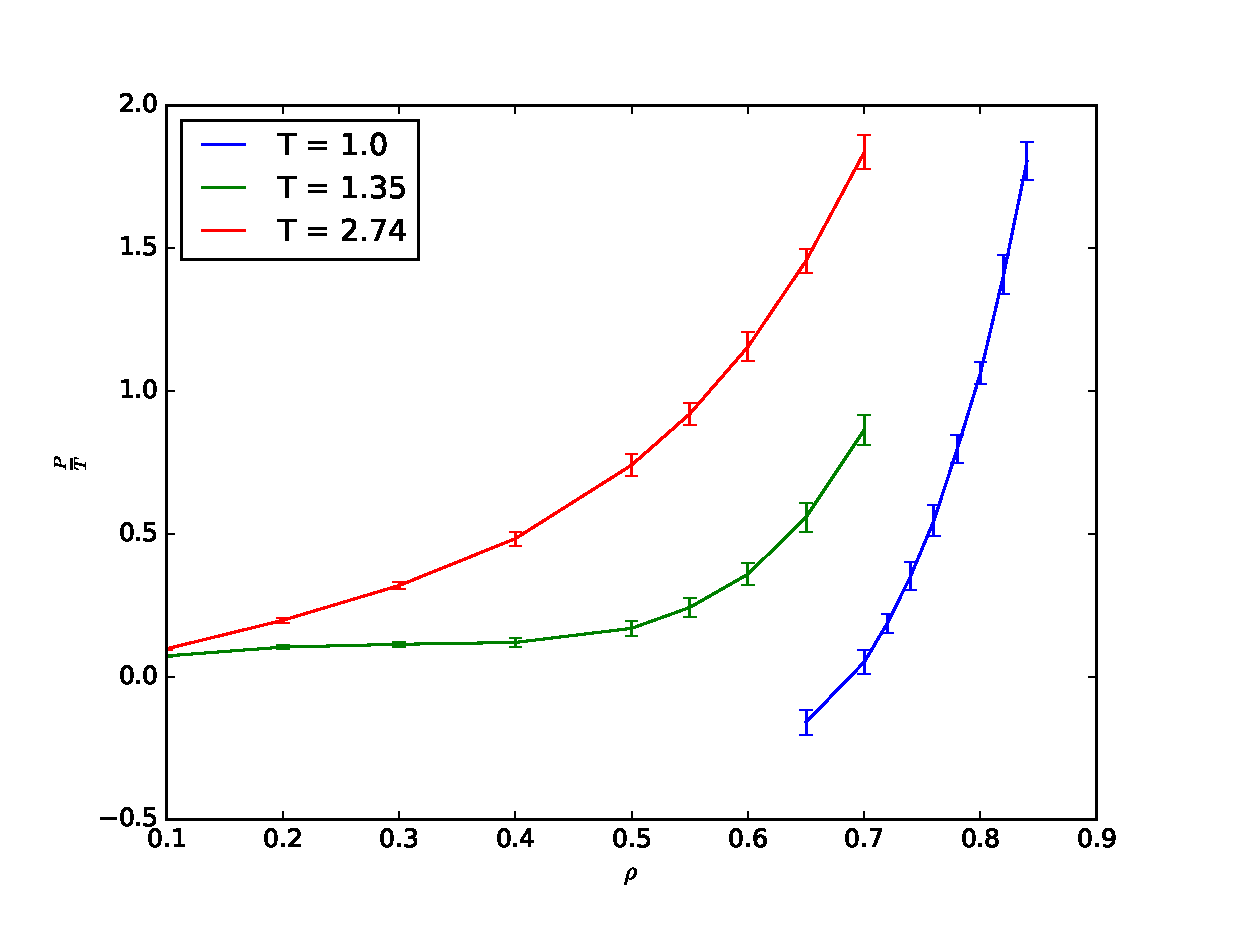
\includegraphics[width=0.6\linewidth]{fig/figure_pressure}
\caption{Plot of the pressure versus the density at different temperatures. Simulations were ran with $N=864$ particles.}
\label{fig:figure_pressure}
\end{figure}


\subsection{Correlation function}
For the correlation function we use the (N, V, T) ensemble, so the velocity is scaled at each timestep as to keep a constant kinetic energy. The correlation function is then calculated using \eqref{eq_correlation}. In Figure~\ref{fig:figure_corr} the results are shown for the gas, solid and liquid phase. The fall off at large distances is due to the finite amount of unit cells taken(6). In the solid phase, \ref{fig:figure_corr_solid} and \ref{fig:figure_corr_solid2}, the effect of temperature is clearly visible in the increase of peak height and decrease of peak width at lower temperature, since the molecules have less oscillation amplitude, giving less spread in $g$. 
\begin{figure}[h]
	\begin{subfigure}[b]{0.48\textwidth}
	\centering
	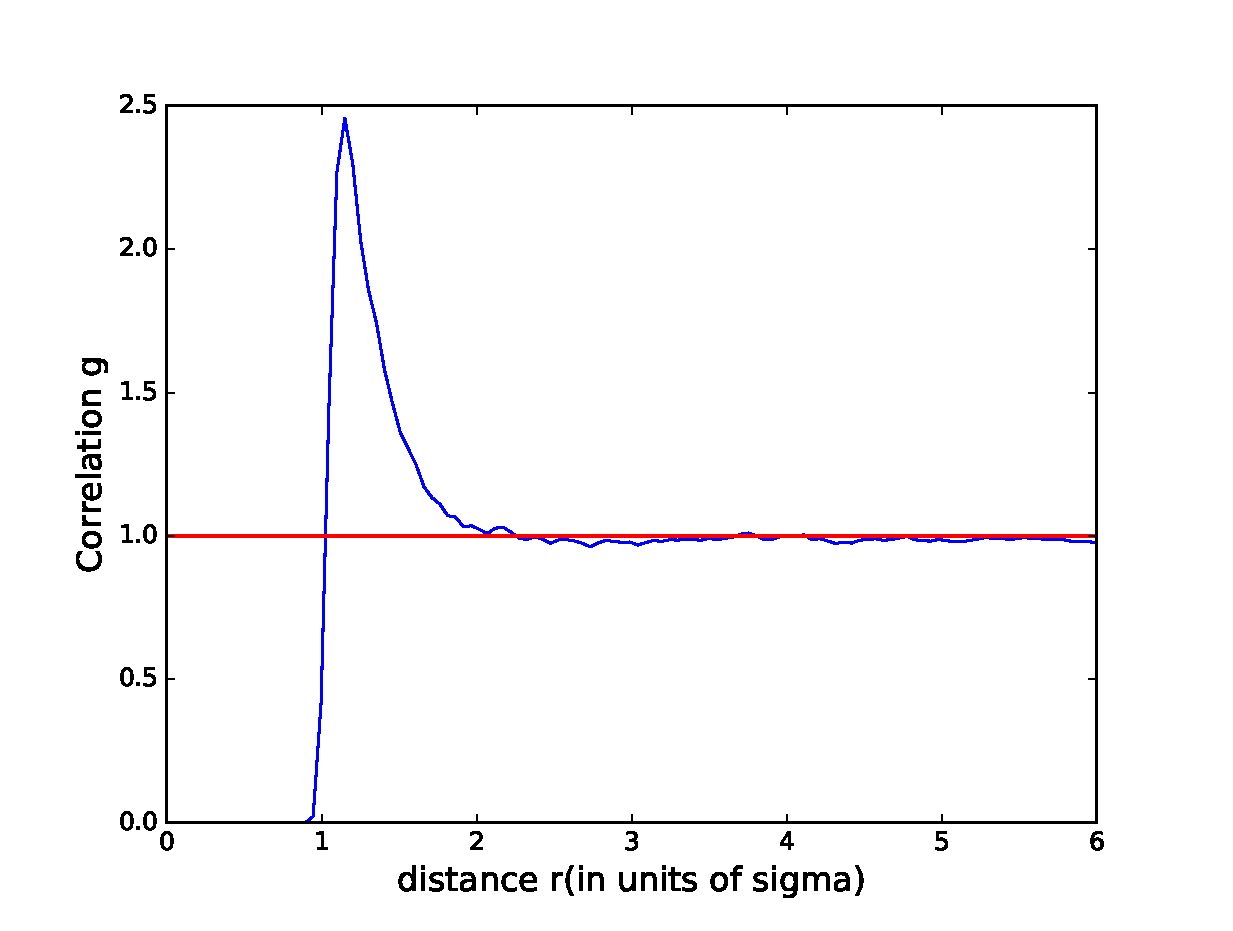
\includegraphics[width=0.9\linewidth]{fig/figure_corr_gas2.eps}
	\caption{$\rho = 0.01$ and $T = 1$}
	\label{fig:figure_corr_gas}
	\end{subfigure}
	\begin{subfigure}[b]{0.48\textwidth}
		\centering
		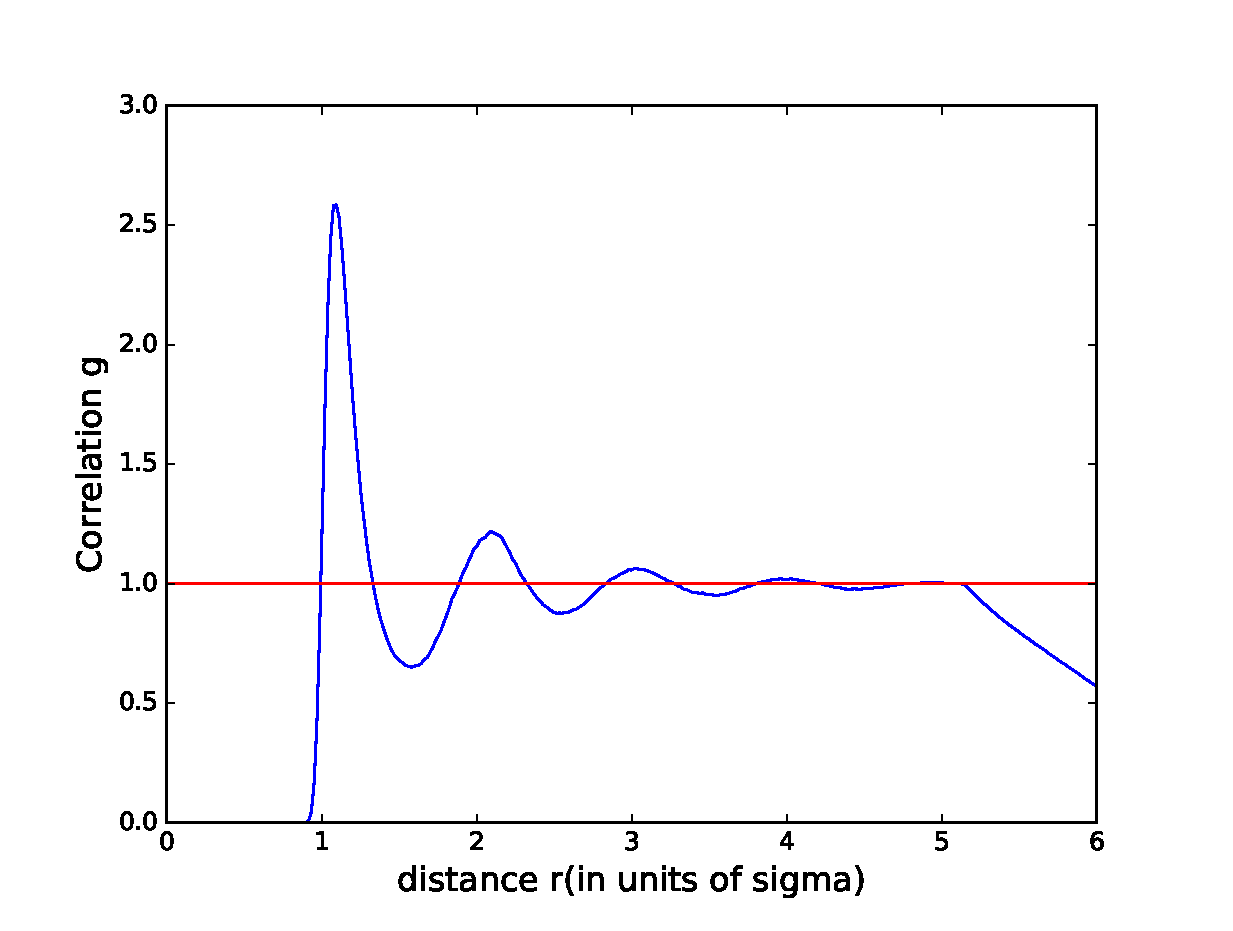
\includegraphics[width=0.9\linewidth]{fig/figure_corr_gas.eps}
		\caption{$\rho = 0.8$ and $T = 1$}
		\label{fig:figure_corr_liquid}
	\end{subfigure}
	
	\begin{subfigure}[b]{0.48\textwidth}
		\centering
		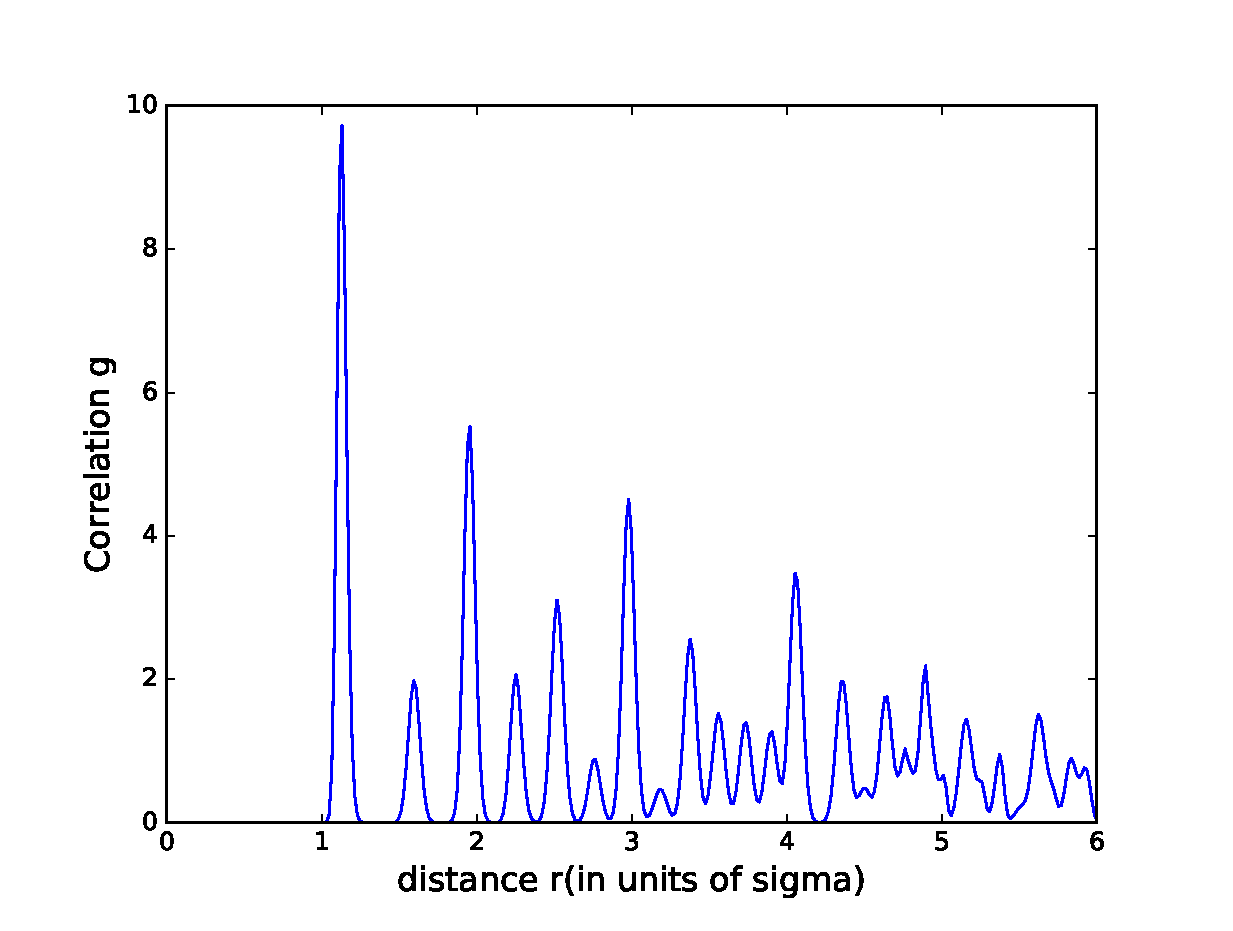
\includegraphics[width=0.9\linewidth]{fig/figure_corr_solid.eps}
		\caption{$\rho = 1$ and $T = 0.1$}
		\label{fig:figure_corr_solid}
	\end{subfigure}
	\begin{subfigure}[b]{0.48\textwidth}
		\centering
		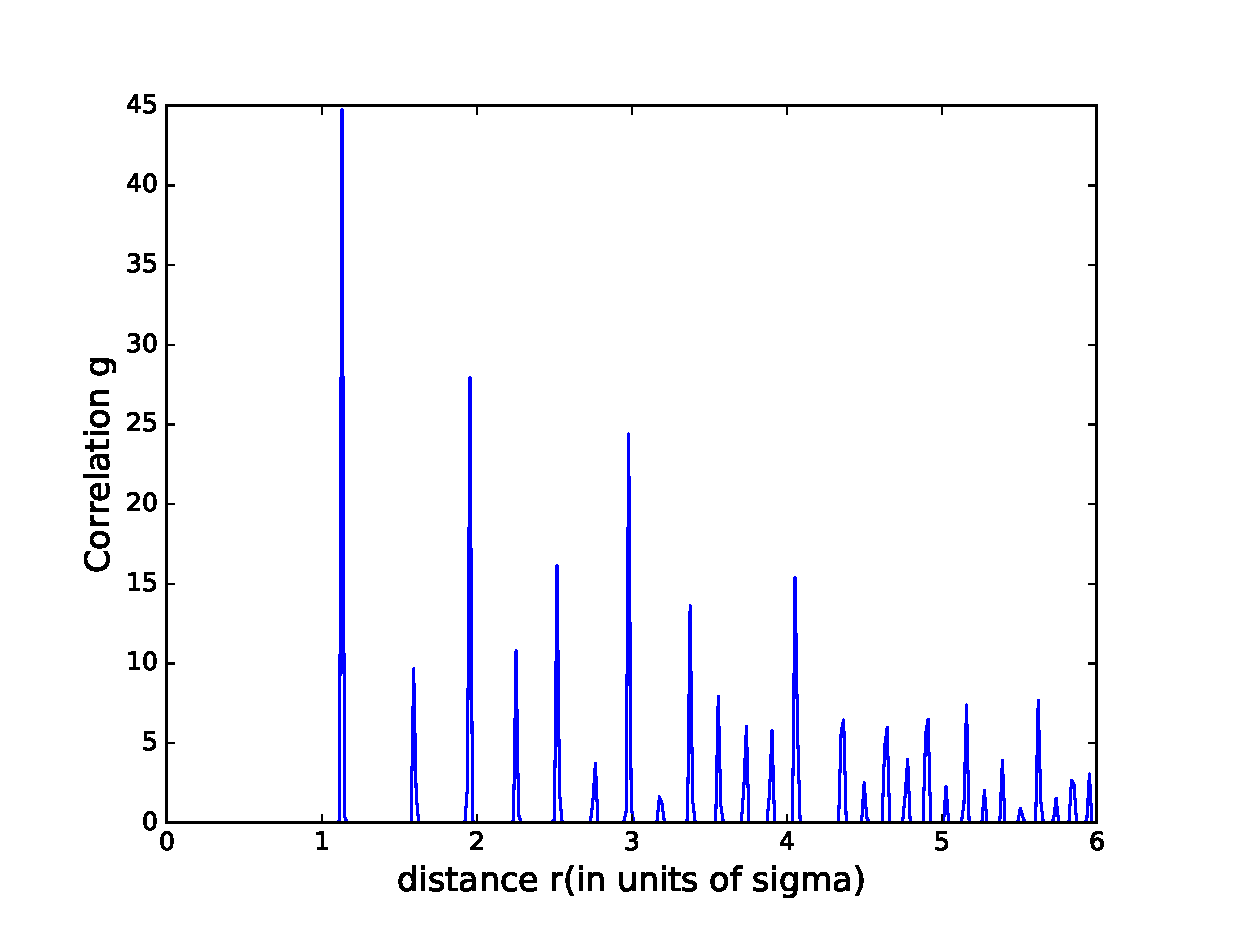
\includegraphics[width=0.9\linewidth]{fig/figure_corr_solid2.eps}
		\caption{$\rho = 1$ and $T = 0.001$}
		\label{fig:figure_corr_solid2}
	\end{subfigure}
	\caption{Shows four evaluations of the correlation function at different densities and Temperature. The gas phase is shown in a, where we clearly see the convergence to 1 for large distances. In b the density a liquid phase is seen. In c and d one clearly sees the discrete peaks corresponding to the FCC structure seen in a solid.}
	\label{fig:figure_corr}
\end{figure}

	
\section{Conclusions}
Using molecular dynamics simulations of Lenard-Jones interacting particles, we were able to obtain equilibrium macroscopic quantities from a microscopic description of the interaction. We effectively simulated Argon, but the method is applicable to any Lenard-Jones interacting substance, and many more macroscopic quantities may be studied if the appropriate statistical relation in known. In particular we verified the computations of the heat capacity at dilute gas and dense solid configurations. Furthermore we have shown a pressure-density relation at different temperatures. Due to the periodic boundary conditions we were not able to resolve two-phase states of argon. Finally we have computed the pair correlation function, which contains local structural information that can be verified in scattering experiments. We obtain characteristic plots for all three phases showing that the Lenard-Jones potential models the interaction for argon in the gas, liquid and solid phase.

%\section{Appendix A - Python Code}\vspace{1em}
%\subsection{Main program}
%\begin{lstlisting}
%%%python CODE HIER
%for i in range(0,10):
%	do cool stuff
%	
%\end{lstlisting}\vspace{1em}\clearpage
%
%
%\section{Appendix B}


\begin{thebibliography}{1}
	%%random voorbeeld boeken
	\bibitem{ref_verlet}
	L.   Verlet  (1967). 
	\newblock Computer  experiments   on   classical   fluids, 
	\newblock Thermodynamical properties of Lennard-Jones molecules,
	\newblock {\em Phys. Rev. 159 (1967), 89 - 103}.
	
	\bibitem{ref_Lebowitz}
	J. L. Lebowitz, J. K. Percus, and L.Verlet, (1967).
	\newblock Ensemble dependence of fluctuations with application,
	to machine calculations,
	\newblock {\em Phys. Rev., 253 (1967), 250 - 254}.
	
	\bibitem{ref_Thijssen}
	J. M. Thijssen (2007).
	\newblock Computational Physics, Ch. 7-8
	\newblock {\em Cambridge University Press}
\end{thebibliography}
	
\end{document}
















